\subsection{Les industriels responsables et la garantie longue durée}


\smallbreak
Contrairement aux garanties légales, la garantie contractuelle ou commerciale est offerte ou non selon la décision du vendeur. C'est pour ça, elle est considérée facultative par rapport aux garanties légales. Le vendeur est obligé de respecter les dispositions qui régissent ces garanties légales, et d'en informer l'acheteur. 
En raison de la garantie commerciale, et en cas de panne,le professionnel s’en charge de la réparation de l’appareil tant que la période de garantie n'est pas terminée. Il peut aussi proposer de remplacer le produit.


\smallbreak
Lorsque le fabricant accorde une garantie pour son produit, celle-ci est nommée « garantie constructeur » ou « garantie fabricant », est aussi supplémentaire. Cette garantie ne devient valide que si le vendeur ne propose pas une garantie commerciale \cite{loigarantie}.
\smallbreak
Cet exemple, on le trouve particulièrement avec la multinationale \textit{Apple} qui fournit une garantie fabricant d’un an \cite{apple}. Cet acte est toute à fais normale car tous les entreprises du domaine électrique et électronique ne offrent que des garanties d’un an, mais \textit{Apple} laisse croire à ses clients que la seule garantie du produit ne durent qu'une seule année depuis la date d'achat du produit,après ce temps le produit n'est plus garantie. Ceci est juste mais l'entreprise américaine joue sur la différence entre la garantie constructeur qui dure un an et les garanties légales qui durent deux ans et plus, et il joue sur l'ignorance de ses clients des garanties qui existe aujourd'hui.


\smallbreak
Aujourd'hui, on commence à voir des entreprises ou des commerçants qui offrent des garanties de longue durée pour leurs produits.
\smallbreak C'est le cas de la société anglaise d’électroménager \textit{Dyson}\footnote{http://www.dyson.com}, qui a proposé des aspirateurs avec une longue garantie de cinq ans. Ce qui veut dire que \textit{Dyson} offre trois ans de garantie de plus, sachant que la garantie constructeur est indiquée en une seule année \cite{dyson}. Normalement pour bénéficier d'une telle garantie, le client devrait payer le prix normal du produit plus une augmentation liée à la garantie,au contraire de la bonne proposition de la marque \textit{Dyson}.


\smallbreak
L’électroménager n'est pas le seul, le domaine automobile, lui aussi a osé de proposer  des garanties de longues durées, par l’intermédiaire de la marque \textit{KIA}. Jusqu’à aujourd'hui, le constructeur automobile sud-coréen avec son modèle \textit{CEE’D}\footnote{http://www.kia.com/fr/fr/modeles/nouvelle-ceed}, reste le seul à proposer une garantie gratuite de sept ans ou 150 000 kilomètres \cite{kia}. Ceci est difficile pour les Européens qui conservent leur voiture pour presque sept ans. Malheureusement, pour les automobilistes, pas toutes les marques ont suivi l’initiative de la marque \textit{KIA}. Ainsi, si le client veux vendre sa voiture pendant la durée de la garantie indiquée dans sept ans, c'est le nouvel acheteur qui profitera du reste de la garantie. Cependant, les constructeurs automobiles européens restent avec des garantie de deux ans.


\smallbreak
On trouve aussi,l'entreprise néerlandaise \textit{Philips} qui a décidé de prendre en compte les conséquences écologiques de l'obsolescence programmée, notamment les produits jetables. Ces dernières années, \textit{Philips} a dirigé son investissement vers  les produits durables. L'un de ces produits durables est l’ampoule \textit{LED}\footnote{http://www.philips.fr/c-m-li/ampoules-led} (Light Emitting Diode), en français la diode électroluminescente ou la diode qui  diffuse de la lumière , cette ampoule a une durée de vie de 25 ans à l'opposée de l'ampoule à incandescence qui dure 2 000 heures (presque 2 ans), elle consomme presque 3 watts d’électricité contrairement à l'ampoule à incandescence qui utilise 25 watts d’électricité \cite{ampoule_inc}. 
\newpage
\smallbreak
Contrairement à \textit{Apple}, le \textit{PhoneBloks}\footnote{https://phonebloks.com} est une des idées innovantes qui vient pour lutter contre l'obsolescence programmée.c'est l'idée d'un designer néerlandais \textit{Dave Hakkens}\footnote{http://davehakkens.nl} qui cherchait à inventer une smartphone complètement personnalisable basé sur un système de brique comme c'est affiché dans l'image au dessous \cite{op_pb}.
\begin{figure}[h]
\begin{minipage}{0.5\linewidth}
\begin{center}
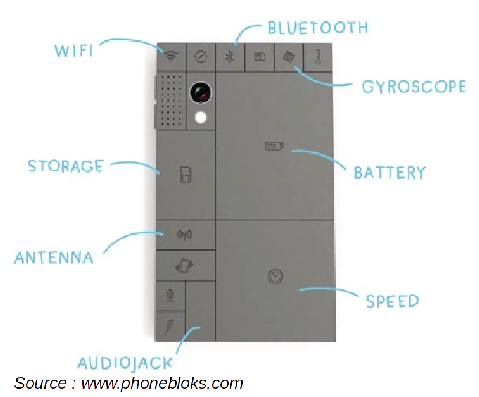
\includegraphics[scale=0.6]{Rsc/phonebloks2.png} 
\end{center}
\end{minipage}
\begin{minipage}{0.5\linewidth}
\begin{center}
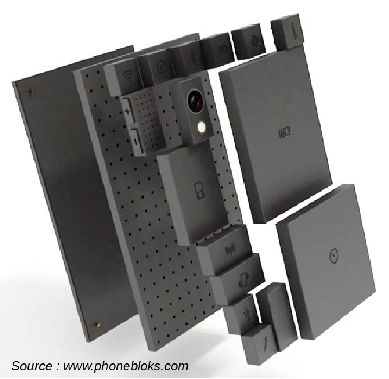
\includegraphics[scale=0.7]{Rsc/phonebloks1.png} 
\end{center}
\end{minipage}
\caption{\scriptsize{Phonebloks : le téléphone qui se monte et se démonte en quelques secondes.}}
\label{phonebloks}
\end{figure}


 Le principe ici, c'est que le téléphone mobile est un ensemble de composants aux différentes fonctions ( Wifi, batterie, GPS, Bluetooth, appareil photo, etc) et en cas de panne d'un composant, il suffit juste de le décrocher et le changer. 
Même si elle toujours dans la phase de conception, l'initiative a connu un grand succès sur les réseaux sociaux.La vidéo de la présentation du \textit{Phonebloks} sur \textit{Youtube} a déjà dépassé les 20 millions de vues \cite{pb_yt}, ce qui prouve qu'il y une vraie volonté des gens qui ont soutenu le projet d'avoir un smartphone avec ses fonctionnalités très puissantes, un smartphone anti-obsolescence. 

%cite{loigarantie}

%cite{apple}

%cite{dyson}

%cite{kia}

%cite{ampoule_inc}

%cite{op_pb}

%cite{pb_yt}


